\documentclass[12pt]{article}

\usepackage{sbc-template}

\usepackage{graphicx,url}

\usepackage{orcidlink}
\usepackage{float}

\usepackage{hyperref}
\usetikzlibrary{arrows.meta,positioning}

\usepackage{tikz}
\usetikzlibrary{positioning}

\usepackage{pgfplots}
\pgfplotsset{compat=1.18}

\usepackage{booktabs}
\usepackage{multirow}
\usepackage{array}

%\usepackage[brazil]{babel}
\usepackage[utf8]{inputenc}

\sloppy
% Ajustes para reduzir espaços verticais e compactar o artigo
\setlength{\textfloatsep}{8pt plus 2pt minus 2pt}
\setlength{\floatsep}{6pt plus 2pt minus 2pt}
\setlength{\intextsep}{7pt plus 2pt minus 2pt}
\setlength{\abovecaptionskip}{3pt}
\setlength{\belowcaptionskip}{2pt}
\setlength{\parskip}{0pt}


\title{Análise de Vulnerabilidades de Memória Assistida por Agentes de IA: Um Estudo Experimental com PHP2Shell\thanks{O código-fonte deste projeto está disponível em:
\url{https://github.com/}}}

\author{Adriano Araújo\inst{1}, Artur Rizzi\inst{1}, Eduardo Aniceto\inst{1}, Izabel Chaves\inst{1}\orcidlink{0009-0008-9198-3909},\\ Pedro Guimarães\inst{1}}

\address{
Departamento de Ciência da Computação -- Instituto de Ciências Exatas e Informática\\
Pontifícia Universidade Católica de Minas Gerais (PUC Minas)\\
30.535-610 -- Belo Horizonte -- Brasil\\
\email{\{1464597, 1568608, 1593221, iopchaves, 1447017\}@pucminas.edu.br}
}

\begin{document}

\maketitle

%-----------------------------------------------
% ABSTRACT
%-----------------------------------------------
\begin{abstract}
Artificial intelligence agents can help automate software vulnerability analysis, but their effectiveness and reproducibility require further evaluation. This work proposes an experimental study of OpenCode for analyzing memory vulnerabilities, using PHP2Shell as a case study. The methodology includes a controlled environment, standardized instructions, and experimental validation of the findings. The gem5 simulator may be used to investigate relevant architectural aspects, depending on software compatibility. The evaluation will consider detection accuracy, false positives and negatives, analysis time, computational cost, and reproducibility. The goal is to identify the capabilities and limitations of AI-assisted vulnerability analysis.
\end{abstract}

%-----------------------------------------------
% RESUMO
%-----------------------------------------------
\begin{resumo}
Agentes de inteligência artificial podem auxiliar na análise de
vulnerabilidades de software, mas sua eficácia e reprodutibilidade
precisam ser avaliadas. Este trabalho propõe um estudo experimental
do OpenCode na análise de vulnerabilidades de memória, utilizando o
PHP2Shell como estudo de caso. A metodologia inclui um ambiente
controlado, instruções padronizadas e validação experimental dos
resultados. O simulador gem5 poderá ser utilizado para investigar
aspectos arquiteturais relevantes, conforme a compatibilidade do
software. A avaliação considerará a precisão na identificação de
falhas, os falsos positivos e negativos, o tempo de análise, o custo computacional e a reprodutibilidade. O objetivo é compreender as capacidades e limitações da análise de vulnerabilidades assistida por IA.
\end{resumo}

\textbf{Keywords:} Artificial intelligence agents; Software security; Memory vulnerabilities; gem5; OpenCode; PHP2Shell.
%-----------------------------------------------
% INTRODUÇÃO
% Deve escrever sobre hipótese, objetivo geral, objetivo específico
%-----------------------------------------------
\section{Introdução}




%-----------------------------------------------
% TRABALHOS RELACIONADOS
% pelo menos 5, mais de 5
%-----------------------------------------------
% \section{Trabalhos Correlatos} -- incorporada à seção anterior
\section{Trabalhos Relacionados}
% Quem vai fazer trabalhos relacionados está em sbc-template.bib

%-----------------------------------------------
% METODOLOGIA
%-----------------------------------------------
\section{Metodologia e Ambiente Experimental}

A pesquisa adota uma abordagem experimental para avaliar a
capacidade do agente de IA OpenCode na análise e validação de
vulnerabilidades de memória no PHP2Shell, tendo a arquitetura
RISC-V como ambiente-alvo. O experimento será dividido em etapas
de preparação, análise assistida, execução controlada e avaliação
dos resultados, conforme apresentado na Figura~\ref{fig:metodologia}.



\begin{figure}[H]
\centering
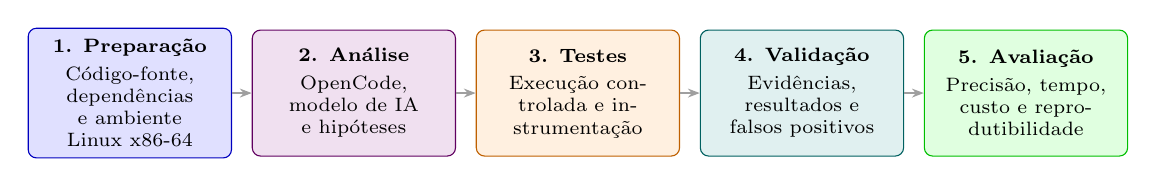
\begin{tikzpicture}[
    node distance=0.25cm,
    etapa/.style={
        rectangle,
        rounded corners=3pt,
        draw=#1!75!black,
        fill=#1!12,
        text width=2.3cm,
        align=center,
        minimum height=1.6cm,
        font=\scriptsize,
        inner sep=4pt
    },
    seta/.style={
        -{Stealth[length=1.5mm]},
        thick,
        draw=gray!75
    }
]

\node[etapa=blue] (a) {
    \textbf{1. Preparação}\\[2pt]
    Código-fonte, dependências e ambiente Linux x86-64
};

\node[etapa=violet, right=of a] (b) {
    \textbf{2. Análise}\\[2pt]
    OpenCode, modelo de IA e hipóteses
};

\node[etapa=orange, right=of b] (c) {
    \textbf{3. Testes}\\[2pt]
    Execução controlada e instrumentação
};

\node[etapa=teal, right=of c] (d) {
    \textbf{4. Validação}\\[2pt]
    Evidências, resultados e falsos positivos
};

\node[etapa=green, right=of d] (e) {
    \textbf{5. Avaliação}\\[2pt]
    Precisão, tempo, custo e reprodutibilidade
};

\draw[seta] (a) -- (b);
\draw[seta] (b) -- (c);
\draw[seta] (c) -- (d);
\draw[seta] (d) -- (e);

\end{tikzpicture}
\caption{Fluxo do procedimento experimental.}
\label{fig:metodologia}
\end{figure}


Nas próximas subseções, são detalhados os recursos utilizados, a configuração do ambiente e os procedimentos adotados para a realização dos experimentos, desde a preparação do sistema até a análise dos resultados obtidos.

\subsection{Ambiente e Procedimento Experimental}

O experimento utilizará o OpenCode, integrado a um modelo de
linguagem, para analisar o código-fonte do PHP2Shell e identificar
possíveis vulnerabilidades de memória. Serão registradas as versões
das ferramentas, as configurações do ambiente e as instruções
fornecidas ao agente, de modo a manter condições consistentes
entre as execuções.

A validação inicial será realizada em ambiente Linux com arquitetura x86-64, utilizada como referência por ser a plataforma documentada para a reprodução da cadeia de exploração do PHP2Shell. A arquitetura ARM64 será considerada para avaliar a portabilidade dos resultados, desde que haja suporte compatível às versões do software e aos componentes necessários. O uso de RISC-V poderá ser investigado posteriormente, mas não será tratado como requisito para a reprodução da vulnerabilidade.

O simulador gem5 será utilizado, quando viável, para executar
programas de teste e investigar aspectos arquiteturais, como ciclos
de processamento, instruções executadas e comportamento da hierarquia de memória. A execução integral do PHP2Shell no simulador dependerá da compatibilidade do sistema operacional, das bibliotecas e dos serviços necessários. Por isso, a validação da vulnerabilidade será distinguida dos experimentos de simulação arquitetural.

Os resultados produzidos pelo OpenCode serão comparados com as
evidências obtidas nos testes controlados, permitindo avaliar a
correção das análises e identificar falsos positivos. Todos os
experimentos serão realizados em ambiente isolado, com registro
das configurações, dos procedimentos e das limitações encontradas.


\subsection{Métricas e Análise dos Resultados}

A avaliação considerará a taxa de sucesso na identificação e
validação das vulnerabilidades, o tempo de análise, o custo
computacional e a reprodutibilidade. A taxa de sucesso será calculada
pela proporção de tarefas validadas em relação ao total de tarefas
válidas, conforme a Equação~\ref{eq:sucesso}.

\begin{equation}
S = \frac{N_s}{N_v}\times 100
\label{eq:sucesso}
\end{equation}

em que $N_s$ representa o número de tarefas bem-sucedidas e $N_v$
o total de tarefas válidas.

O tempo será medido durante as execuções, enquanto o custo
computacional considerará o consumo de memória, o tempo de CPU e,
quando aplicável, o custo de utilização do modelo. A reprodutibilidade
será verificada por meio de repetições sob as mesmas condições,
comparando as respostas do OpenCode com as evidências obtidas nos
testes. Os resultados serão organizados em tabelas e gráficos,
destacando acertos, erros e limitações observadas.

%-----------------------------------------------
% RESULTADOS
%-----------------------------------------------
%\section{Resultados}

%-----------------------------------------------
% CONCLUSÃO
%-----------------------------------------------
%\section{Conclusão}

%-----------------------------------------------
% TRABALHOS FUTUROS
%-----------------------------------------------
%\section{Trabalhos Futuros}


%-----------------------------------------------
% USO DE IA
%-----------------------------------------------
%\section{Uso de IA}

%\newpage

\bibliographystyle{sbc}
\bibliography{sbc-template}

\end{document}